\chapter{AST XML Generation Pass}
\section{ENUM-Based Visitor's Design Pattern}
In Tasks 3,4,5 we need to traverse each and every node and perform some specific operation. Each node has a \verb!type! which is an enum value. We use an enum-based visitors pattern  to identify the type of a node (subtree)  and carry out the required operations.


The design requires us to have an interface  \verb!Vistor! holding a visitor method for each type.  \verb!Visitor! is implemented by the concrete classes to ensure that all the nodes in an AST are visited and acted upon accordingly.

\textbf{A diagram showcasing the design pattern is given below.}

\begin{landscape}
\begin{figure}[H]
    \centering
        
    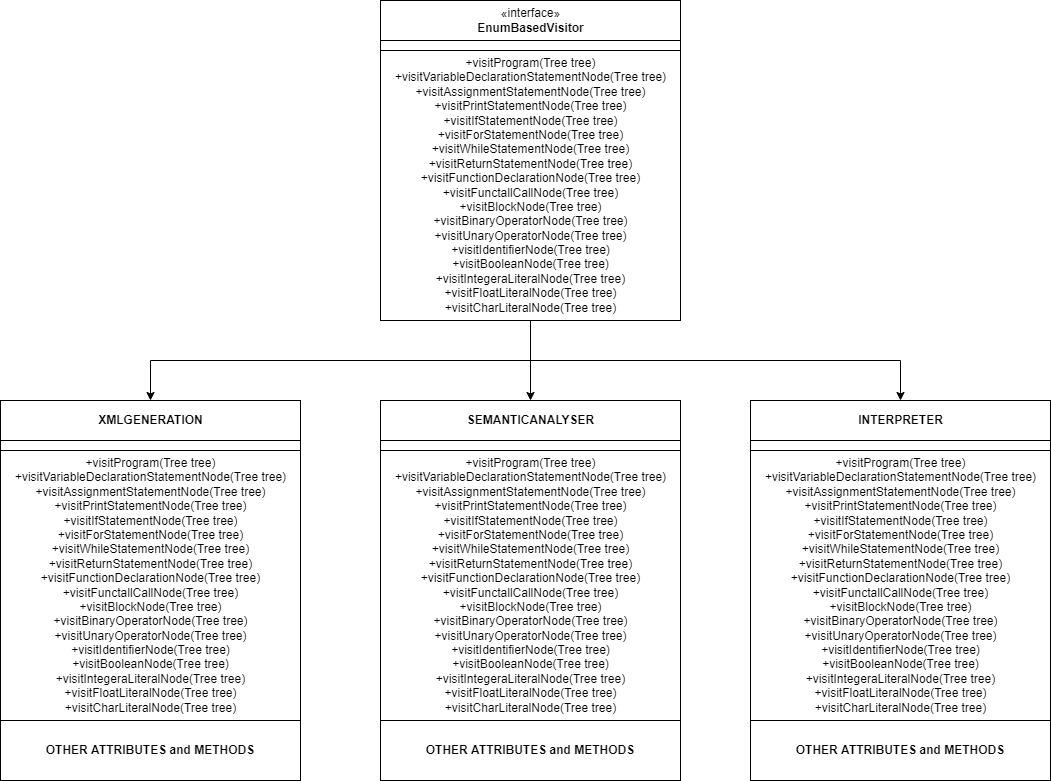
\includegraphics[scale=0.5]{Task345/images/UML.png}
    
    \caption{\emph{XmlGeneration,Semantic Analyser and Interpreter} are concrete implementations of interface EnumVisitor.}
    \label{fig:enum based visitors design pattern}
\end{figure}
\end{landscape}

\section{Design}
\label{sec:design task 3}
We want to generate a string representation of an abstract tree. We use XML representation. Now each node corresponds to a different subtree and each tree corresponds to a different XML tag. Hence we use the visitor's design pattern and use the required visitor method to generate the appropriate XML tags and content.

Consider the AST in figure \ref{fig:tiny-lang-ast} an XML representation is given below.
\begin{lstlisting}[caption=XML representation of AST shown in figure \ref{fig:tiny-lang-ast}]
<TinyLangProgram>
    <function declaration>
        <id type="FLOAT"> Sq <\id>
        <parameters>
            <id type="FLOAT"> x <\id type>
        <\parameters>
        <block>
          <return statement>
            <binary Op>
                <id type="FLOAT"> x <\id type>
                <id type="FLOAT"> x <\id type>
            <\binay Op>
         <\return statement>
        <\block>
    <\function declaration>
    <print>
        <function call>
            <id>Sq<\id>
            <parameters>
                <actual parameter>
                    <id>x<\id>
                <\actual parameter>
                <actual parameter>
                    <id>x<\id>
                <\actual parameter>
            <\parameters
        <\function call>
    <\print>
<TinyLangProgram>
\end{lstlisting}

Class\verb! XMLGeneration! implements interface \verb!Visitor! as shown in figure \ref{fig:enum based visitors design pattern}.


Apart from the visitor methods the class also holds  these attributes and methods:
\begin{itemize}
    \item \verb!String xmlRepresentation! -> the actual XML of the program in consideration
    \item \verb!int indentation! -> keeps track of the current indentation level and updates accordingly
    \begin{itemize}
        \item we have a method which generate an indentation as a sequence of tabs (\verb!0x09!) spaces where the number of white spaces correspond to \verb!indentation! 
\begin{lstlisting}[caption=Get current indentation]
getCurrentIndentation():
    String indentation = ""
    for(i<0;i<this.identation;i++):
        indentation+="    "
        return indetation
\end{lstlisting}
    \end{itemize}
    \item Constructor is given by:
\begin{lstlisting}[caption=XmlGeneration Constructor]
XmlGeneration(Tree tree):
    //visit the whole abstract syntax tree is 
    //equivalent to visiting a program
    visitProgram(tree)
\end{lstlisting}
\end{itemize}
\subsection{visit Program and Statement(s)}
The root node of any AST is of type \verb!AST_PROGRAM_NODE! hence we start any XML Generation with tag \verb!<TinyLangProgram>!. 


The children of the program node are statement subtrees (as described in section \ref{sec:statement trees ast}). 

Hence for each child we call a method \verb!visitStatment(tree)! which identifies the type of tree and calls the required \verb!visitor! accordingly so the right tags and content are produced. 
\begin{lstlisting}[caption=PSEUDOCODE of \emph{visitProgram(tree)}]
xmlRepresentation+=getCurrentIndentation()+"<TinyLangProgram>\n"
//we indent next body
indentation++
for(child : currentTree.children)
    visitStatement(child)
//unindent (tags attain same level of indentaion)
indentation--
xmlRepresentation+=getCurrentIndentation()+"<\TinyLangProgram>\n"
\end{lstlisting}
\textbf{Note:} opening and closing tags attains the same level of indentation

Method \emph{visitStatement(tree)} call another other visitor method that visit nodes of statement type based on the type of the node.

\begin{lstlisting}[caption=
PSEUDOCODE for \emph{visitStatement(tree)},label=listing:visit statement tree]
If tree/node is of type:
AST_VARIABLE_DECLARTION_NODE -call-> visitVariableDeclarationNode(tree)
AST_ASSIGNMENT_NODE -call-> visitAssignmentNode(tree)
AST_PRINT_STATEMENT_NODE -call-> visitPrintStatementNode(tree)
AST_IF_STATEMENT_NODE -call-> visitIfStatementNode(tree)
AST_FOR_STATEMENT_NODE -call-> visitForStatementNode(tree)
AST_WHILE_STATEMENT_NODE -call-> visitWhileStatementNode(tree)
AST_RETURN_STATEMENT_NODE -call-> visitReturnStatementNode(tree)
AST_FUNCTION_DECLARATION_NODE -call-> visitFunctionDeclarationNode(tree)
AST_BLOCK_NODE -call-> visitBlock(tree)
otherwise -> throw exception unexpected 
\end{lstlisting}


Let us take a look at an example of a statement type visitor method : \verb!visitVariableDeclaration(Tree tree)!.

A variable delcaration statement tree has 3 children. The first child of type \verb!AST_TYPE_NODE! which correspond to the type of the expression, the second child is  of \verb!AST_IDENTIFIER_NODE! which corresponds to the name given to the variable, and the third child is an expression subtree. Visitor methods whose type is related to expression are discussed in section \ref{sec:visit expression visitor}
.

We use this structure of the tree to generate its corresponding XML representation:
\begin{lstlisting}[caption=XML of variable declaration statement subtree]
<variable declaration>
    <id type=TYPE> variable name<\id>
    .... | some
     .... | expression
    .... | body
<\variabld declaration>
\end{lstlisting}




The PSEUDCODE  to build a XML representation of the variable declaration statement is as follows .
\begin{lstlisting}[caption=PSEUDCODE of \emph{visitVariableDeclarationNode(Tree tree)}]
xmlRepresentation += getCurrentIndentation ()+"<variable declaration>\n"
//we indent for next body 
indentation ++
//get type from first child and identifier from second child
xmlRepresentation += getCurrentIndentation ()+"<id type="+tree.getChildren().get(0).value+">"+ tree.getChildren().get(1).value+"<\id>\n"
//visit epxression -> third child 
visitExpression(tinyLangAst.getChildren().get(2))
// unindent (tags attain same level of indentaion )
indentation --
xmlRepresentation += getCurrentIndentation ()+"<\variable declaration>\n"
\end{lstlisting}


\textbf{Note:} opening and closing tags attains the same level of indentation

\textbf{
The other statement visit methods are implemented similar to as shown in listing above.
}

\subsection{visit Expression(s)}
\label{sec:visit expression visitor}
Almost all statements have an expression subtree. So we need to decide what the type of expression is so we produce the right nested tags and expressions.

Whenever a call to an expression visit method needs to be made,we first call \verb!visitExpression(Tree tree)!, and visit expression calls the required visit method according the the type of the tree. For example if the tree is of type \verb!AST_UNARY_OPERATOR_NODE! then we call $visit $ 

In general we have the following:
\begin{lstlisting}[caption=PSEUDOCODE for \emph{visitExpression(Tree tree)},label=listing:expression visit]
AST_BINARY_OPERATOR_NODE -call-> visitBinaryOperatorNode(tree)
AST_UNARY_OPERATOR_NODE -call-> visitUnaryOperatorNode(tree)
AST_BOOLEAN_LITERAL_NODE -call-> visitBooleanLiteralNode(tree)
AST_INTEGER_LITERAL_NODE -call-> visitIntegerLiteralNode(tree)
AST_FLOAT_LITERAL_NODE -call-> visitFloatLiteralNode(tree)
AST_CHAR_LITERAL_NODE -call-> visitCharLiteralNode(tree)
AST_IDENTIFIER_NODE -call-> visitIdentifierNode(tree)
AST_FUNCTION_CALL_NODE -call-> visitFunctionCallNode(tree)
otherwise -> throw exception unexpected
\end{lstlisting}

For example for a binary operator tree we have that the root of the tree is a binary tree whose root is a binary operator and its 2 children are expression tree in its own right. Therefore the 2 intended tags inside a binary operation expression will be expression tags in their own right.

The visitor \verb!visitBinaryOperatorNode(tree)! is defined recursively as follows.
//we obtain value of binary operator and append it to opening tag
\begin{lstlisting}[caption=PSEUDOCODE for visitBinaryOperatorNode(Tree tree)]
xmlRepresentation += getCurrentIndentation ()+"<binary Op="+tree.value+">\n"
//check for 2 children (we expect 2 children)
if(tree.getChildren().size!=2) 
    throw unexpected
//we indent for next body 
indentation ++
//visit first child (an expression)
visitExpression(tree.getChildren().get(0));
//visit first child (an expression)
visitExpression(tree.getChildren().get(1));
// unindent (tags attain same level of indentation )
indentation --
xmlRepresentation += getCurrentIndentation ()+"<\variable declaration>\n"
\end{lstlisting}


\verb!visitFunctionCallNode(Tree tree)! and \verb!visitUnaryOperatorNode(Tree tree)! has an analogous recursive definition to one given in the listing above.

The implementations of the other expression visitor methods i.e. visitBooleanLiteralNode (tree), visitIntegerLiteralNode (tree), visitFloatLiteralNode (tree), visitCharLiteralNode(tree) and visitIdentifierNode (tree) is \verb!trivial! and they act as the \textbf{base case} for the recursion.




\section{Implementation in Java}
All the design decisions mentioned in \ref{sec:design task 3} are implemented as shown in listing \ref{listing:xmlGeneration}
\section{Testing}
Consider Program 1,2,3 discussed in testing Tasks 1,2,3 their XML representations are given below:
\begin{figure}[H]
    \centering
    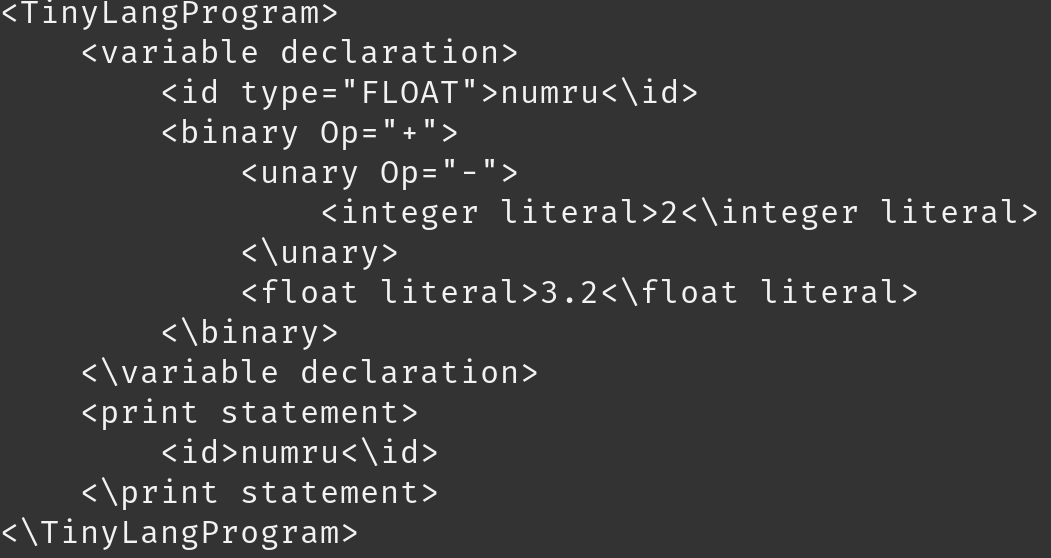
\includegraphics[scale=0.5]{Task345/images/xmlOutput1.png}
    \caption{XML representation for program 1}
    \label{fig:xml tree 1}
\end{figure}
\begin{figure}[H]
    \centering
    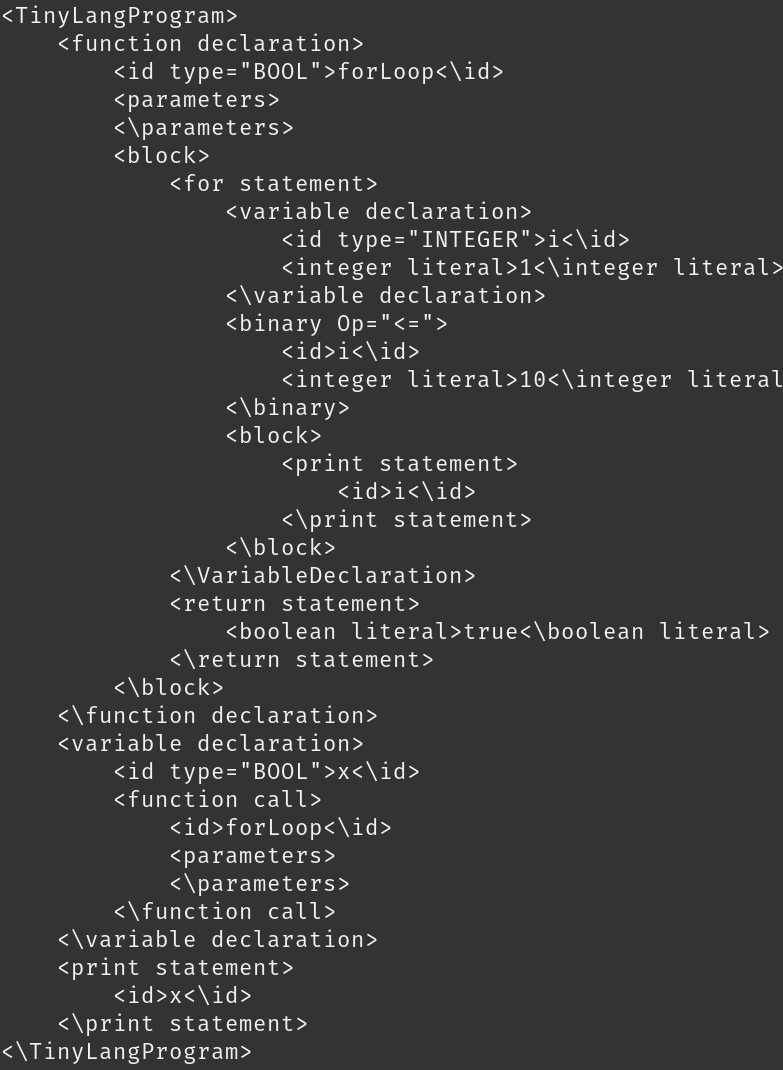
\includegraphics[scale=0.5]{Task345/images/xmlOutput2.png}
    \caption{XML representation for program 2}
    \label{fig:xml tree 2}
\end{figure}
\begin{figure}[H]
    \centering
    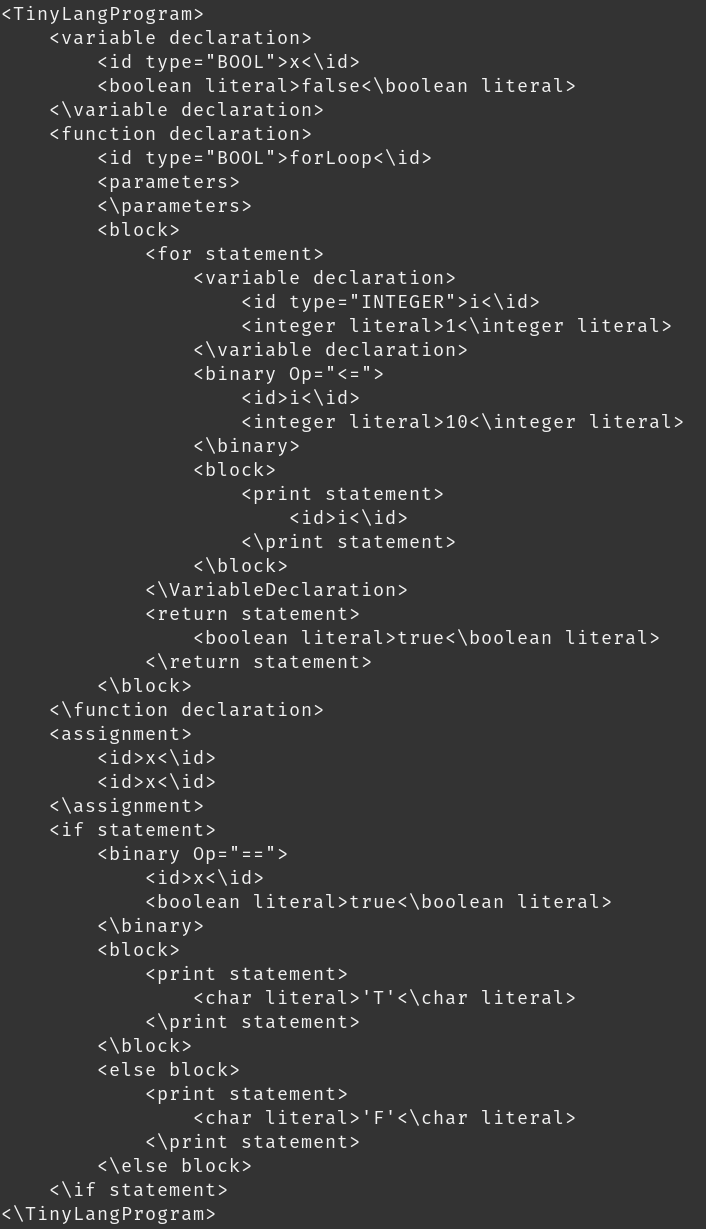
\includegraphics[scale=0.5]{Task345/images/xmlOutput3.png}
    \caption{XML representation for program 3}
    \label{fig:xml tree 3}
\end{figure}





\chapter{Semantic Analysis}
\verb!SemanticAnalyser! class implements visitor methods to traverse the $AST$ to ensure that the program semantics are correct before moving to the interpretation tree.

\section{Design}
\label{sec:design semantic}
\subsection{Scopes}
We  keep track of scopes. 


A global scope is created in the constructor and then we visit the program tree. A global scope is destroyed after a  successful visit  of the program tree without any errors. If we manage to reach the end of the global scope then we conclude that the program is semantically correct.
\begin{lstlisting}[caption=PSEUDOCODE : constructor (start of program traversal)]
//create new scope 
st.push()
//traverse the program
visitProgram(tree)
//end scope
st.pop
print("program semantically correct")
\end{lstlisting}

A new local scope is created  and destroyed when control enters and leaves a block respectively. Therefore each time we visit a block we push a new scope to the symbol table and at the end of the visit we pop out the scope.
\begin{lstlisting}[caption=PSEUDOCODE : \emph{visitBlockNode(Tree tree)}]
//create new scope
st.push();

-> add parameters of functions if any in scope
-> clear currentFunctionParameters
-> visit all statements in block

//end scope
st.pop();
\end{lstlisting}

\textbf{Note:} Whenever a new function declaration is made we update a map  \verb!currentFunctionParameters! defined in semantic analyser class as $Identifier \rightarrow Type$. So whenever we enter a new scope from the function declaration we have a reference to the identifier and type of function parameters.

\textbf{Note:} A program is visited in a similar way to Task 3 and we  deduce what visit method to use based on the  type of the root node. 


\subsection{Variable re-declaration}
Note a scope keeps a mapping between a variable name and a type. 






\textbf{Note:}
\begin{lstlisting}[caption=The same variable name can be used in different scopes]
{
    let a : float = 5;
    print a;
    {
        let a : char = 'a'; 
        print a;
    }
}
\end{lstlisting}
The first print method will print \verb!5! and the second print method will print \verb!'a'!.




We check if a variable is already declared in current scope by checking if it is mapped to some type in that scope via function \verb!isVariableNameBinded(String varName)!. 

\begin{lstlisting}[caption=PSUEDOCODE : checking if a variable is already declared in currentScope (in method visitVariableDeclarationNode(Tree tree)) ]
//second child of the tree corresponds to identifier
Tree identifier = tree.getChildren().get(1)
//check if name of identifier is already declared in current scope
if(st.isVariableNameBinded(identifier.getAssociatedNodeValue())==true)
    throw exception
\end{lstlisting}

\subsection{Function Overloading}

This section describes how we allow for function overloading and described the visitor method: 



We allow for function overloading by defining the signature of a function.

A function signature is made up by the name of the function and the types of the parameters. For example,
\begin{enumerate}[(a)]
\item fn Sq (int x , float y) -> int  {...}
\item  fn Sq (int a , float b) -> char {...}
\item fn Sq (float x , float y) -> float {...}
\end{enumerate}

\textbf{(a)} and \textbf{(b)} have the same signature, \textbf{(b)} and \textbf{(c)} do not have the same signature.

This is implemented by constructing a \verb!FunctionSignature! class which contains \verb!String functionName! and a stack of type \verb!Type! where \verb!Type! is an \verb!ENUM! defined by constants \verb!BOOL!,\verb!INTEGER!,\verb!CHAR! and \verb!FLOAT!).

Each unique instance of \verb!functionSignature! is a unique  function signature. 

In each scope we have a mapping between \verb!functionSignature! and enum \verb!Type!.
\begin{lstlisting}[caption=PSEUDOCODE of isFunctionAlreadyDefined(FunctionSignature signature) inside class \emph{SCOPE}]
//check if a function is declared within a scope
boolean isFunctionAlreadyDefined(FunctionSignature signature):
    return functionDeclarationMap.containsKey(signature)
\end{lstlisting}










\textbf{Any scope can contain function declaration and once a scope dies that function is undeclared.}

When declaring a new function we check if a function with the same signature is already declared in the current and even outer scopes (for variable we only check the current scope i.e. variable can be declared in new scopes even if they are already declared in outer ones). Therefore in \verb!visitFunctionDeclaration(Tree tree)! we obtain the function name and the function parameter types from the children and we check  if they are defined 

\begin{lstlisting}[caption=PSEUDOCODE: checking if a function is already declared in all scopes]
for(Scope scope : st.getScopes()):
    if(scope.isFunctionAlreadyDefined(new FunctionSignature(functionName, functionParameters))):
        throw error
\end{lstlisting}
\begin{lstlisting}[caption=PSEUDOCODE:  if a function is not  declared in all scopes we push it to current scope via class SymbolTable]
st.insertFunctionDeclaration(new FunctionSignature(functionName, functionParameters))
\end{lstlisting}


\subsection{Type Checking}
\subsubsection{Visit Expression}

A semantic analyser class has an attribute \verb!Type currentExpressionType! to make reference to the type of the current expression. 


We visit an expression to find the  type value returned by the expression an update \verb!currentExpressionType! for \textbf{type checking.}

An expression can take many forms. Whenever we have to visit an expression tree we call  \verb!visitExpression()!. This method calls the required visitor according to the node/expression type as discussed in \ref{listing:expression visit}

We check the type of the expression as follows.
\begin{itemize}
    \item If expression is of type \textbf{binary expression.}
    \verb!visitBinaryOperatorNode(Tree tree)! is implemented as follows. We get hold on what the operator is by checking the value associated with node/tree. Since the 2 children are expression in their own right we make a recursive call to \verb!visitExpression(Tree)! to obtain the type of both operands. Then we perform type checking and update \verb!currentExpressionType! accordingly.
    \begin{itemize}
        \item If the operator is \verb!'and'! or \verb!'or'! we check that both operands types are bool else we throw exception. We  also set  \verb!currentExpressionType! to bool. 
        \item Else If the operator is \verb!+!, \verb!-!, \verb!/! and \verb!*!  we check that both operands types is of numeric type (float or int) else  throw exception. If one of the operands is of type float we set \verb!currentExpressionType! to float otherwise we set it to int.
        \item Else If the operator is \verb!<!, \verb!>!, \verb!<=! and \verb!>=!  we check that both operands types is of numeric type (float or int) else  throw exception. We also set \verb!currentExpressionType! to bool.
        \item Else If the operator is \verb!==!, \verb|!=| we check that both operands are of the same type otherwise we throw error. We set \verb!currentExpressionType! to bool. 
        \item Else we throw \textbf{exception unrecognised operator}
    \end{itemize}
  
  
    \item If expression is of type \textbf{unary expression.}
    \begin{itemize}
        \item We check that the unary operator is \verb!+!, \verb!-!, or \verb!not! otherwise we throw exception. \item The only child of the unary operator tree is an expression in its own right. We visit the unary tree child and update \verb!currentExpressionType()!.
        \item If current expression type is of numeric type (i.e. integer or float) we check if the operator is \verb!-! or \verb!+! otherwise we throw error.
        \item If current expression type is of bool type we check if the operator is \verb!not! otherwise we throw error.
    \end{itemize}
  
    \item If expression is of type \textbf{integer literal node expression.}
    \begin{itemize}
        \item We just set \verb!currentExpressionType! to int.
    \end{itemize}
    \item If expression is of type \textbf{float literal expression.}
    \begin{itemize}
        \item We just set \verb!currentExpressionType! to float.
    \end{itemize}
    \item If expression is of type \textbf{boolean literal expression.}
    \begin{itemize}
        \item We just set \verb!currentExpressionType! to boolean.
    \end{itemize}
    \item If expression is of type \textbf{char literal expression.}
    
       \begin{itemize}
        \item We just set \verb!currentExpressionType! to char.
    \end{itemize}
    \item If expression is of type \textbf{identifier}
    \begin{itemize}
        \item Start traversing the scopes from the innermost scopes to check in which most inner scope the identifier is declared. Then we set \verb!currentExpressionType! to the type of the variable in that scope.
    \end{itemize}
 
    \item If expression is of type \textbf{function call}
    \begin{itemize}
        \item     Get hold of the function signature by checking function name and each type of the actual parameters (expression).
    
    Start traversing scopes to see where the function is defined and use method \verb!getFunctionType(signature)! in that scope to obtain the type of the function and set \verb!currentExpressionType! to it.
    \end{itemize}


\end{itemize}




\subsubsection{Considerations}
We allow integer literals to resolve to float type. 

E.g. let x:float=5; is \textbf{allowed}.

We do not allow float literals to resolve to integer type. E.g. let x:int=5.01; is \textbf{not allowed}.


\begin{itemize}
    \item \textbf{Variable Declaration.}
    \begin{itemize}
        \item We visit the expression (3rd child) then we check if \verb!currentExpressionType! is the same as the type of the variable. Note that by the consideration  shown above the type of var can be float and the type of expression can be int but not the other way around.
    \end{itemize}
    \item \textbf{Function Declaration.}
    \begin{itemize}
        \item We check that a function returns.
        
        
     \textbf{A check to see if the type of expression it returns matches the type of the function was not implemented.}
    \end{itemize}
    \item \textbf{Assignment.}
    \begin{itemize}
        \item Similar to the case of variable declaration but we obtain the type of the variable by searching from the innermost scope, where the variable is declared and obtain its type by calling \verb!getVariableType(identifier)! in that scope instance.
    \end{itemize}

\end{itemize}






\subsection{Checking if a function returns}
A function must reach a return statement. This can be tricky when we have branching.

A predicate function returns(Tree tree) takes a block tree and returns true if a return statement is reached unconditionally.

The method is built recursively to deal with statements which have blocks. Otherwise if a statement is a simple statement (i.e. no blocks) and is not a return statement then returns(statement) is guaranteed to be false.

For the recursive parts we consider the following cases:
\begin{itemize}
    \item For an if statement we check if we have both the normal block and the else block else the statement is not guaranteed to return. Then we we check if both block returns.
    \item A block/else-block is returning if it contains a statement that returns.
    \item For for and while loops we check if the block returns.
\end{itemize}


The PSEUDOCODE is given below.

\begin{lstlisting}[caption=PSEUDOCODE: \textbf{Defining predicate \emph{returns(Tree tree)}}]
Base Case (trivial case) tree represents a return statement :
if(tree.type=AST_RETURN_STATEMENT):
    return true
//(Recursive case) if statement is a block we check if one of the statements inside the
//block returns
if(tree.type=AST_BLOCK_NODE):
    for(Tree statement : tree.getChildren()):
        //if one statement within block
        //returns the whole block returns
        if(returns(statement)):
            return true
        
)
//(Recursive case) if statement is an else block we check if one of the statements inside
// the else block returns
if(tree.type=AST_ELSE_BLOCK_NODE):
    for(Tree statement : tree.getChildren()):
        //if one statement within block
        //returns the whole block returns
        if(returns(statement)):
            return true
)

//(Recursive case) if statement is an if statement block has an else block
(i.e. if statement tree has 3 children)
//and check if the block and else block contains
//a returning function
if(tree.type=AST_IF_STATEMENT_NODE):
    if(tree.getChildren().size=3):
    //check if children block treee and else block tree returns
        return returns(tree.getChildren().get(1) and returns(tree.getChildren().get(2))
//(Recursive case) check that block inside for/while loops is returning 
if(tree.type=AST_FOR_STATEMENT_NODE):
    //block statement is last child 
    //a for statement can have different amount 
    //of children
    return returns(tree.getChildren().get(tree.getChildren().size-1))
if(tree.type=AST_FOR_STATEMENT_NODE):
    //block statement is second child
    return returns(tree.getChildren().get(1))
// (base case) otherwise in all other cases 
else:
    return false
\end{lstlisting}




\section{Implementation in Java}
\begin{itemize}
    \item The implementation class \verb!FunctionSignature! whose instance are used to check if functions are already declared is given in listing \ref{listing:functionsignature}
    \item The implementation class \verb!Scope! and the data structures and methods required to make reference to the variables,functions is given in listing \ref{listing:scope}
    \item The implementation of class symbol table which holds a stack of scopes, and method to insert/destroy scopes etc is given in listing \ref{listing:symboltable}
    \item All points discussed through the design section \ref{sec:design semantic} are implemented as shown in listing \ref{listing:semanticanalyser}
    \end{itemize}
    
    
    
\section{Testing}

Let us test some program that are is semantically incorrect and ensure that an appropriate exception is produced.

\begin{itemize}
    \item A program with a function that is not guaranteed to return (conditional branching).
\begin{lstlisting}[basicstyle=\tiny,caption=Program 4]
//a function must always return,this function is not guaranteed to return
fn notGuranteedToReturn(x:char)->bool{
     if(x=='a'){ return true; }
     else{ 
         //conditional branching 
         if(x=='b'){ return true; }
     else{
             if(x=='c'){ return true; }
             else{
        		//no return statement in this block
        		print 'c';
             }  
        }     
     }
}
\end{lstlisting}
    The following exception is thrown:
    \begin{figure}[H]
        \centering
        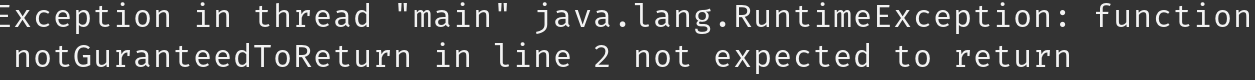
\includegraphics[scale=0.7]{Task345/images/funcNotExpectedToReturn.png}
        \caption{Exception}
        \label{fig:exception function not expected to return}
    \end{figure}
    
    
        
    
    \item Expecting a bool expression 
\begin{lstlisting}[basicstyle=\tiny,caption=Program 5]
//expecting an expression type of bool
// i+10 is not of type bool -> error
let i:int=1;
while(i+10){
	print i;
}
\end{lstlisting}

    The following exception is thrown:
    \begin{figure}[H]
        \centering
        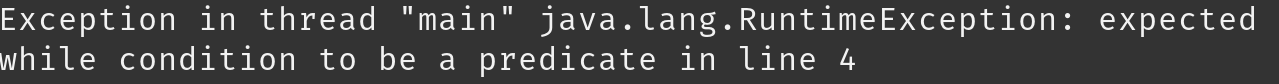
\includegraphics[scale=0.7]{Task345/images/typeCheckingError.png}
        \caption{Exception}
        \label{fig:exception function not expected to return}
    \end{figure}
    
    \item A program where 2 variables with the same name are defined in the same scope.
    
\begin{lstlisting}[basicstyle=\tiny,caption=Program 6]
fn notNice(x:char)->bool{
	let x:bool=false;
	//error variable x already declared
	let x:int=5;
	print x;
}

\end{lstlisting}

    The following exception is thrown:
    \begin{figure}[H]
        \centering
        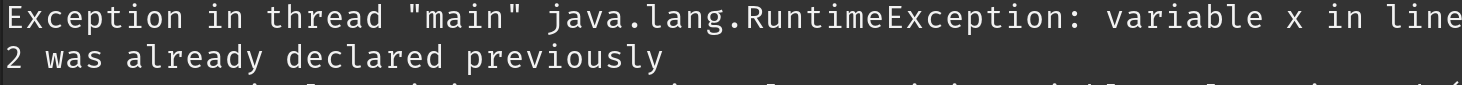
\includegraphics[scale=0.7]{Task345/images/errorVariableRedclar.png}
        \caption{Exception}
        \label{fig:exception function not expected to return}
    \end{figure}

    \item A function redeclared inside same program (same signature)
    
    
    

\begin{lstlisting}[basicstyle=\tiny,caption=Program 7]
fn notNice(x:char)->bool{
	fn notNice(x:char)->int{
		return 0;
	}
	return notNice('a');
}
\end{lstlisting}


   The following exception is thrown:
    \begin{figure}[H]
        \centering
        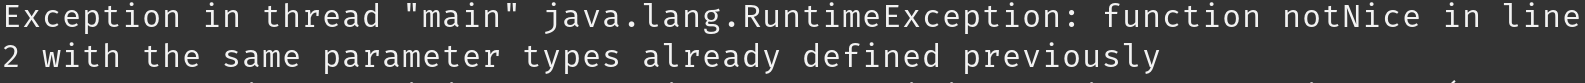
\includegraphics[scale=0.7]{Task345/images/errorFuncRedclar.png}
        \caption{Exception}
        \label{fig:exception function not expected to return}
    \end{figure}
    
        \item A program that is semantically correct with \textbf{Function Overloading} -> a program containing program with same identifier but having parameter of different types
\begin{lstlisting}[basicstyle=\tiny,caption=Program 8       ]
fn nice(x:int)->float{
	fn return2()->int{
		return 2;
	}
	return x+return2();
}
fn nice(x:float)->float{
	fn return3()->int{
		return 3;
	}
	return x+return3();
}
print nice(1);
print nice(1.0);
\end{lstlisting}


The program is semantically correct and the following output is thrown when interpreted (Task 5):
\begin{figure}[H]
    \centering
    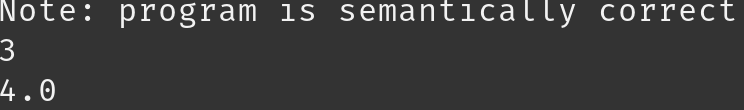
\includegraphics[scale=1]{Task345/images/semantically-correct-program.png}
    \caption{Exception}
    \label{fig:exception function not expected to return}
\end{figure}    
    
\end{itemize}

\chapter{Interpreter}
\label{sec:interpreter design}
\section{Design}
This task is similar to task 4. We need to have an appropriate symbol table to keep track of scopes. In this task we also require that the symbol table also holds values so we can  simulate an interpreter which executes the test program.


\subsection{Scope}
The following functionality was added in classes \verb!SemanticAnalyser! and \verb!Scope!.
\begin{itemize}
    \item In each scope we keep a mapping between variable names and their values \verb!Map<String,String> variableValues!. A mapping between a function signature and its block tree \verb!Map<FunctionSignature,Tree> functionBlock!. A mapping between function signatures and their respective parameter names \verb!Map<FunctionSignature,Stack<Strign>> functionParameterNames!.
   
    \item  Methods \verb!addVariableValue(String varName,String varValue)! to map a value to a variable, \verb!addFunctionBlock(FunctionSignature functionSignature,Tree block)! to map a block tree to a function and \verb!addFunctionParameterNames(FunctionSignature fs,!
    \verb!Stack<String> names)! to map parameter identifiers to function.
\end{itemize}

\textbf{
Ensure that program semantics are correct  to ensure that a program can be interpreted correctly.} A call to semantic analyser is made in constructor of the interpreter via \verb!new SemanticAnalyser(treeIntermediateRepresentation)!.



\subsection{Evaluation of expressions}
An interpreter class has values : \verb!Type currentExpresionType! and \verb!String currentExpressionValue! to keep track of the value and type of the latest evaluated expression.

Whenever a statement  needs to evaluate an expression (i.e. has an expression subtree) we call method \verb!visitExpression(Tree tree)! which then makes a call to another visitor method base on the current node type/type of expression (see listing \ref{listing:expression visit}).
\begin{itemize}
    \item If current node type is of type \verb!AST_BINARY_OPERATOR_NODE! a call to \verb!visitBinaryOperatorNode(tree)! is made. 
    \begin{itemize}
        \item  We keep hold of the operator which is given by the node value. The left and right operands (2 children) are expression trees in their own right. A recursive call \verb!visitExpression(tree)! is made on both operands to obtain their type and value (by seeking the values of \verb!currentExpressionType! and \verb!currentExpressionValues!). Then we update the value of \verb!currentExpressionType! and \verb!currentExpressionValue! based on the binary operator and the values and types of both operands. For example consider the following scenarios:
        \begin{itemize}
            \item Operator is \verb!"+"! and both operators are of type int with values \verb!"1"! and \verb!"3"!. We set the \verb!currentExpressionType! to int and the \verb!currentExpresionValue! to \verb!String.valueOf(Int.parseInt("1")+Int.parseInt("3"))="4"!
               \item \textbf{(Implicit Typecasting Case)} Operator is \verb!"*"! and one  operators  of type int  and the other is of type float with values \verb!"2"! and \verb!"3.3"!. We set the \verb!currentExpressionType! to float and the \verb!currentExpresionValue! to \verb!String.valueOf(Float.parseFloat("2")*!
               \verb!Float.parseFloat("3.3"))="6.6"!
               \item (\verb!currentExpressionType! \textbf{depends on value case})
               \item Operator is \verb!"=="! and both operands are of the same type otherwise we throw error unexpected. We set the \verb!currentExpressionType! to the type of the operands and the \verb!currentExpresionValue! to \verb!"true"! if both operands have the same value (i.e. \verb!value1.equals(value2)!), otherwise we set it to \verb!false!.
        \end{itemize}
    \end{itemize}
 
        \item If current node type is of type \verb!AST_UNARY_OPERATOR_NODE! a call to \verb!visitUnaryOperatorNode(tree)! is made.
         \begin{itemize}
        \item A unary tree has an expression subtree as its child. We call \verb!visitExpression(Tree tree)! on  its child to update \verb!currentExpressionValue! and \verb!currentExpressionType!. If the current expression type is \verb!int! or \verb!float!  we check if the unary operator is \verb!-!. If it is we update the value of the current expression e.g. \verb!currentExpressionValue=String.valueOf(-1*Integer.!
        \verb!parseInt(currentExpresssionValue))!. Else if the current expression is of type bool we check i f the unary operator is \verb!not! we update current expression value to false if it was true and to true if it was false.
        Else we throw error unexpected.
        \end{itemize}
        
         \item If current node type is of type \verb!AST_BOOLEAN_LITERAL_NODE! a call to \verb!visitBooleanLiteralNode(tree)! is made.
         \begin{itemize}
             \item When we visit a node of type boolean literal we set the current expression type to bool and the current expression value to the value associated with the node (true or false).
         \item Nodes of type \verb!AST_INT_LITERAL!, \verb!AST_FLOAT_LITERAL! and \verb!AST_CHAR_LITERAL! are dealt with in a similar way.
       
         \end{itemize}
         
            \item If current node type is of type \verb!AST_IDENTIFIER_NODE! a call to \verb!visitIdentifierNode(tree)! is made.
           \begin{itemize}
               \item We get hold on the value/identifier name of the node. We search  the most inner scope the variable name is declared by calling \verb!scope.isVariableNameBinded(identifier)! in each scope. We obtain the type  and value of the variable at that scope by calling methods \verb!scope.getVariableType(identifier)! and \verb!scope.getVariableName(identifier)! and we update the \verb!currentExpressionValue! and \verb!currentExpressionType!.
           \end{itemize}
           \item If current node type is of type \verb!AST_FUNCTION_CALL_NODE! a call to \verb!visitFunctionCallNode(tree)! is made.
           \begin{itemize}
                \item Class interpreter have 2 other data structures \verb!parameterTypes! and \verb!parameterValues!.
               \item For a function call we obtain the name of the function and the expression, and we visit all the actual parameters/expressions to obtain the \verb!currentExpressionType! and push it to \verb!paramaterTypes! and obtain \verb!currentExpressionValue! and push it to \verb!parameterValues! 
               \item We start searching the scopes to find where the function is declared. We check if a function is declared in a scope using the instance method \verb!isFunctionAlreadyDefine(new FunctionSignature(functionName,parameterValues))!
              \item  The interpreter also has a data structure \verb!parameterNames! so when we visit a block node corresponding to the function we can declare the local function variables.
              \item We obtain the block corresponding to a declared function in some scope by using the instance method \verb!getBlock(Function Signature)!
           \end{itemize}
         
\end{itemize}

\subsection{Evaluation of statements}
A program is a sequence of statements, for each statement we call method \verb!visitStatement(Tree tree)! which
then makes a call to another visitor method base on the current node
type of statement (see listing \ref{listing:visit statement tree}).


\begin{itemize}
    \item If current node type is of type \verb!AST_VARIABLE_DECLARATION_NODE! a call to \verb!visitVariableDeclarationNode(tree)! is made.
    \begin{itemize}
        \item We obtain the type and var name from the first  and second children respectively. We visit the expression tree (3rd child) to update \verb!currentExpressionType!  and \verb!currentExpressionValue!. We push the variable type,name and value in current scope.
        \begin{itemize}
            \item \verb!st.insertVariableDeclartaion(varName,varType)!
            \item \verb!st.insertVariableValue(varName,currentExpressionValue)!
        \end{itemize}
    \end{itemize}
        \item If current node type is of type \verb!AST_ASSIGNMENT_NODE! a call to \verb!visitAssignmentNode(tree)! is made.
        \begin{itemize}
            \item Obtain the identifier name from the value associated with the first child. Visit visit the expression (2nd child) to update \verb!currentExpressionType! and \verb!currentExpresssionValue!. Then we search the inner most scope where the variable is declared and update the varaible value by calling instance method
            \verb!addVariableValue(varName, currentExpressionValue)! which updates the value of of the map $varName \rightarrow varValue$ in the innermost scope.
        \end{itemize}
    \item If current node type is of type \verb!AST_PRINT_STATEMENT_NODE! a call to \verb!visitPrintStatementNode(tree)! is made. 
    \begin{itemize}
        \item \textbf{This allows us to test the program by verifying the output.}
        \item we visit expression tree (first child) and update the current expression value then we print the value of the current exprssion
        
        \verb!System.out.println(currentExpressionValue)!
    \end{itemize}
     \item If current node type is of type \verb!AST_IF_STATEMENT_NODE! a call to \verb!visitIfStatementNode(tree)! is made.
     \begin{itemize}
         \item We visit the expression fir child and update\verb!currentExpressionValue! and \verb!currentExpressionType!. We check if the current expression.
         \item If the \verb!currentExpressionValue! is true we visit the block node.
         \item If the \verb!currentExpressionValue! is false we visit the else block (we also check that an else block exists i.e. we check also that if statement has 3 children). 
     \end{itemize}
        \item If current node type is of type \verb!AST_FOR_STATEMENT_NODE! a call to \verb!visitForStatementNode(tree)! is made.
        \begin{itemize}
            \item To deal with the different cases the for loop was encoded as a while loop.
            \item When the for loop has no variable declaration and assignment (only an expression) we keep repeating the statements in the block statements and update the expression (to update truth value). PSEUDOCODE code is given below.
\begin{lstlisting}[caption={\emph{for(;expression;)\{...\}} encoded as while loop}]
while(currentExpressionValue.equals("true")){
    visitBlockNode(block)
    //update current expression value
    visitExpression(expression);
}
\end{lstlisting}
            \item When the for loop has both a variable declaration and an assignment the first child is a variable declaration statement so we call \verb!visitVariableDeclarationNode(first child subtree)! to declare the variable in current scope and we visit the expression (2nd child) to update \verb!currentExpressionValue! to check if it is true or false.
            Then for loop is encoded in a while loop as given in the following PSEUDOCODE.
\begin{lstlisting}[caption=\emph{for(declaration;expression;assignment)\{...\}}]
while(currentExpressionValue="true"){
    //4th child correspond to block node
    visitBlockNode(4th child)
    //visit assignment node (updation)
    visitAssignment(third child)
    //update truth value
    visitExpression(2nd child)
}
\end{lstlisting}
\item After the while loop stops then we delete the variable assigned in the while loop from the current instance by calling instance method \verb!st.deleteVariable!
\end{itemize}
\item \textbf{We deal with the other cases i.e. case where we have no assignment and case where we have no variable declaration using a similar strategy.}

\item If current node type is of type \verb!AST_WHILE_STATEMENT_NODE! a call to \verb!visitWhileStatementNode(tree)! is made. A while statement is easily implemented using a while loop itself.
\begin{lstlisting}[caption=encoding of while loop]
    //first child corresponds to expression -> update current expression value
    visitExpression(first child)
    while(currentExpressionValue.equals("true")):
        visitBlockNode(block);
        visitExpression(expression);
\end{lstlisting}
 \item If current node type is of type \verb!AST_RETURN_STATEMENT_NODE! a call to \verb!visitReturnStatementNode(tree)! is made.
 \begin{itemize}
     \item All we do is just update \verb!currentExpressionType! and \verb!currentExpressionValue! by visiting the expression tree (1st child).
 \end{itemize}
      \item If current node type is of type \verb!AST_FUNCTION_DECLARATION_NODE! a call to \verb!visitFunctionDeclarationNode(tree)! is made.
    \begin{itemize}
        \item We obtain the type, name and block tree of the function from the first, second and fourth child respectively. We traverse the formal parameters tree (3rd child) to obtain a a stack \verb!functionParameterTypes! and a stack \verb!functionParameterNames! of function parameter types and names respectively.
        \item 
        We insert the function declaration in current scope by calling the instance method \verb!st.insertFunctionDeclaration(new!
        \verb!FunctionSignature(functionName,functioNParameters)!. Similarly we map the function parameter names and the function block to the function signature in the current scope.
    \end{itemize}
   \item If current node type is of type \verb!AST_BLOCK_NODE! a call to \verb!visitBlockNode(tree)! is made.
   \begin{itemize}
       \item We create a new local scope \verb!st.push()! when we start traversing the block subtree and destroy scope \verb!st.pop! when we leave.
       \item Also before we start traversing the statements we declare the function parameters inside the newly created local scope.
       \item After they have been declared we clear any data structures in class \verb!Intepreter! holding information about formal parameters.
   \end{itemize}
\end{itemize}

\section{Implementation in Java}
All the design decisions implemented in section \ref{sec:interpreter design} are implemented in Java as shown in listing \ref{listing:interpreter}

\section{Testing}
Let us interpret some programs
\begin{itemize}
    \item Printing \verb!HelloWorld! character by character.
\begin{lstlisting}[basicstyle=\tiny,caption=helloworld.tl]
print 'H';
print 'e';
print 'l';
print 'l';
print 'o';
print 'W';
print 'o';
print 'r';
print 'l';
print 'd';
\end{lstlisting}
Interpreter produces the following output:
\begin{figure}[H]
    \centering
    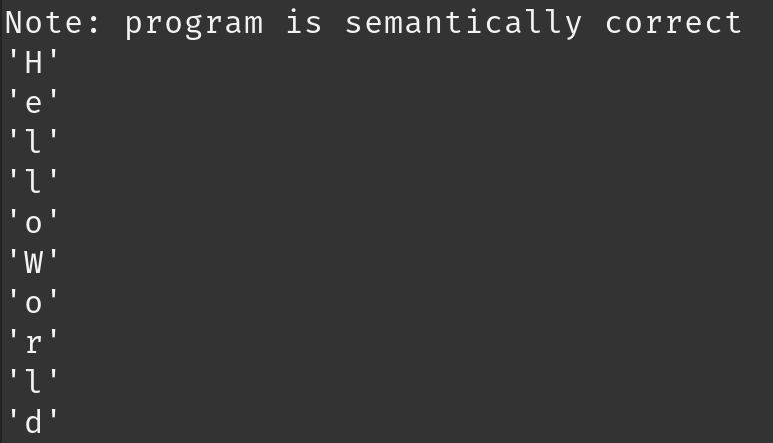
\includegraphics[scale=0.8]{Task345/images/helloworld.png}
    \caption{Output of helloworld.tl}
    \label{fig:output helloworld}
\end{figure}
\item \textbf{(Recursion)} Find the 12th Fibonacci number (1,1,2,3,5,8,13,21,34,55,89,\textbf{144},....)  
\begin{lstlisting}[basicstyle=\tiny,caption=fibonacci.tl]
fn fib(n:int)->int
{
	if(n<=1) {return n;}
	else {return (fib(n-1)+fib(n-2));}
}
print fib(12);
\end{lstlisting}
Interpreter produces the following output:
\begin{figure}[H]
    \centering
    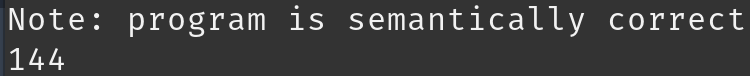
\includegraphics[scale=0.8]{Task345/images/fib.png}
    \caption{Output of fibonacci.tl}
    \label{fig:output fibonacci}
\end{figure}
\item We consider variable values in the most inner scope.
\begin{lstlisting}[basicstyle=\tiny,caption=variables variables.tl]
{
    let a:int=5;
    print a;
    {
          let a:int=6;
          print 6;
	  {
	       let a:int=7;
	       print 7;
	  }
    }
}
\end{lstlisting}
Interpreter produces the following output:
\begin{figure}[H]
    \centering
    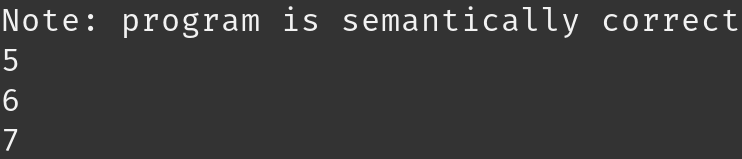
\includegraphics[scale=0.8]{Task345/images/variables-output.png}
    \caption{Output of variables.tl}
    \label{fig:output fibonacci}
\end{figure}
\item Some recursive operators on $\mathbb{N}$.
\begin{lstlisting}[basicstyle=\tiny,caption= recursive.tl]
fn add(a:int,b:int)->int{
    if(b==0){return a;}
    else{
    	return add(a+1,b-1);
    }
}
//reuse add function
fn multiply(a:int,b:int)->int{
    if(b==0){return 0;}
    else{
    	return a+multiply(a,(b-1));
    }
}
//a^b, reuse multiply function
fn power(a:int,b:int)->int{
    if(b==0){return 1;}
    else{
    	if(b==1){return a;} else{
    	return a*power(a,b-1);
    	}
    }
}
print add(5,3);
print multiply(5,3);
print power(5,3);
\end{lstlisting}
\begin{figure}[H]
    \centering
    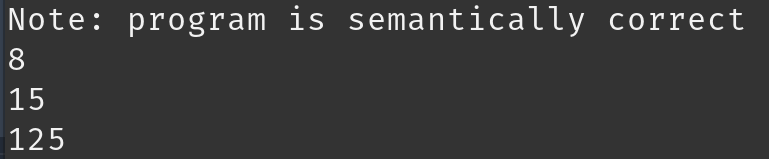
\includegraphics[scale=0.8]{Task345/images/recursive.png}
    \caption{Output of recursive.tl}
    \label{fig:output fibonacci}
\end{figure}
\item A program that uses the previous functions to work out the summation $\sum\limits_{k=0}^{5} k^2+(2*k+2)=2+5+10+17+26+37=97 $


\begin{lstlisting}[basicstyle=\tiny,caption=sum.tl]
fn add(a:int,b:int)->int{
    if(b==0){return a;}
    else{
    	return add(a+1,b-1);
    }
}
//reuse add function
fn multiply(a:int,b:int)->int{
    if(b==0){return 0;}
    else{
    	return a+multiply(a,(b-1));
    }
}
//a^b, reuse multiply function
fn power(a:int,b:int)->int{
    if(b==0){return 1;}
    else{
    	if(b==1){return a;} else{
    	return a*power(a,b-1);
    	}
    }
}
let sum:int=0;
for(let i:int=0;i<=5;i=i+1){
	let a:int = power(i,2);
	
	let b:int = multiply(i,2);
	let c:int = add(b,2);
	let d:int = add(a,c);
		print d;
	sum=sum+d;

}
print sum;
\end{lstlisting}
\begin{figure}[H]
    \centering
    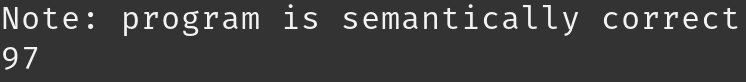
\includegraphics[scale=1.2]{Task345/images/sum.png}
    \caption{Output of sum.tl}
    \label{fig:output fibonacci}
\end{figure}
\end{itemize}
\section{Future implementation}
I wish to add the following features to the next iteration of tinylang:
\begin{itemize}
    \item Allow use of more complex data structures such as string and arrays.
    \item Have more expressive printing methods.
    \item Allow a program to make references to other programs.
\end{itemize}


